\documentclass[]{article}

%opening
\title{4F13 Probabilistic Machine Learning - Gaussian Processes}
\author{Lawrence Tray \\ St John's College}

%packages
\usepackage[margin=0.5in]{geometry}
\usepackage{graphicx}
\usepackage{amsmath}
\usepackage{amssymb}
\usepackage{hyperref}
\usepackage{caption}
\usepackage{subcaption}
\usepackage{parskip}
\usepackage{listings}

%package setup
\graphicspath{{./img/}}
\DeclareMathOperator*{\argmax}{arg\,max}
\DeclareMathOperator*{\argmin}{arg\,min}

%custom commands
\newcommand{\dft}{\mathcal{F}}
\newcommand{\idft}{\mathcal{F}^{-1}}
\newcommand{\Xcal}{\mathcal{X}}
\newcommand{\Ncal}{\mathcal{N}}
\newcommand{\cmplx}{\mathbb{C}}
\newcommand{\Lcal}{\mathcal{L}}
\newcommand{\figwidth}{0.6\linewidth}

%section numbering
\renewcommand{\thesubsection}{\thesection.\alph{subsection}}

\begin{document}

\maketitle

\begin{abstract}
\end{abstract}

\section{Introduction}

\section{Questions}
\subsection{Squared Exponential Covariance Function}

We start with a simple squared exponential (SE) covariance function. As we start by working in one dimension this is necessarily isotropic. The covariance function is given by:

\begin{equation}
k_{SE}(x, x') = \nu^2 \exp\left\{- \frac{(x-x')^2}{2\lambda^2}\right\}
\label{eqn:covSEiso}
\end{equation}

The hyperparameters are $\nu$ and $\lambda$ which control the baseline variance level and length scale of variation respectively. We load in the training data from \textit{`cw1a.mat'} and train a GP model, with zero mean and covariance function given by equation \ref{eqn:covSEiso}. We assume a Gaussian likelihood function with noise variance $\sigma^2$ such that $P(y|\mu) = \Ncal(y; \mu, \sigma^2)$, where $\mu$ is the associated mean. We train the model hyperparameters by minimising the negative log marginal likelihood - denoted $\Lcal$. This is achieved through the commands in listing \ref{lst:opt}.

\begin{lstlisting}[frame=single, caption={Hyperparameter optimisation}, label={lst:opt}]
cov = [-1, 0]; lik = 0;
hyp = struct('mean', [], 'cov', cov, 'lik', lik);
hyp2 = minimize(hyp, @gp, -100, @infGaussLik, meanfunc, covfunc, likfunc, x, y);
\end{lstlisting}

\begin{table}[!h]
\centering
\begin{tabular}{c | c c | c c}
	\textbf{Parameter} & \textbf{A Initial} & \textbf{A Final} & \textbf{B Initial} & \textbf{B Final} \\ \hline
	$\log \lambda$           & -1                 & -2.054           & -0.45              & 2.085            \\
	$\lambda$                & 0.368              & 0.128            & 0.638              & 8.045            \\
	$\log \nu$         & 0                  & -0.109           & 0                  & -0.363           \\
	$\nu$              & 1                  & 0.897            & 1                  & 0.696            \\
	$\log \sigma$      & 0                  & -2.139           & 0                  & -0.411   \\
	$\sigma$           & 1                  & 0.118            & 1                  & 0.663    \\ \hline
	$\Lcal$            & 92.9               & 11.9             & 92.5               & 78.2  
\end{tabular}
\caption{Hyperparameter optimisation (log values included as reported by gpml toolbox)}
\label{tab:hyp-opt}
\end{table}

Table \ref{tab:hyp-opt}, scenario A shows one example of optimising the parameters\footnote{The negative log marginal likelihood $\Lcal$ is not a hyperparameter but rather a function evaluated on the dataset given the current setting of the hyperparameters. It is included in this table for reference.} to minimise the negative log-likelihood. This yields a predictor as in figure \ref{fig:1a}. The 95\% error bound is computed by $[\mu(x) - 2\sigma(x), \mu(x) + 2\sigma(x)]$. In other words, as $y \sim \Ncal(\mu(x), \sigma(x)^2)$, there is a 95\% chance of $y$ falling within two standard deviations of the mean (all evaluated at a specific $x$).

\begin{figure}[!h]
	\begin{subfigure}{0.5\linewidth}
		\centering
		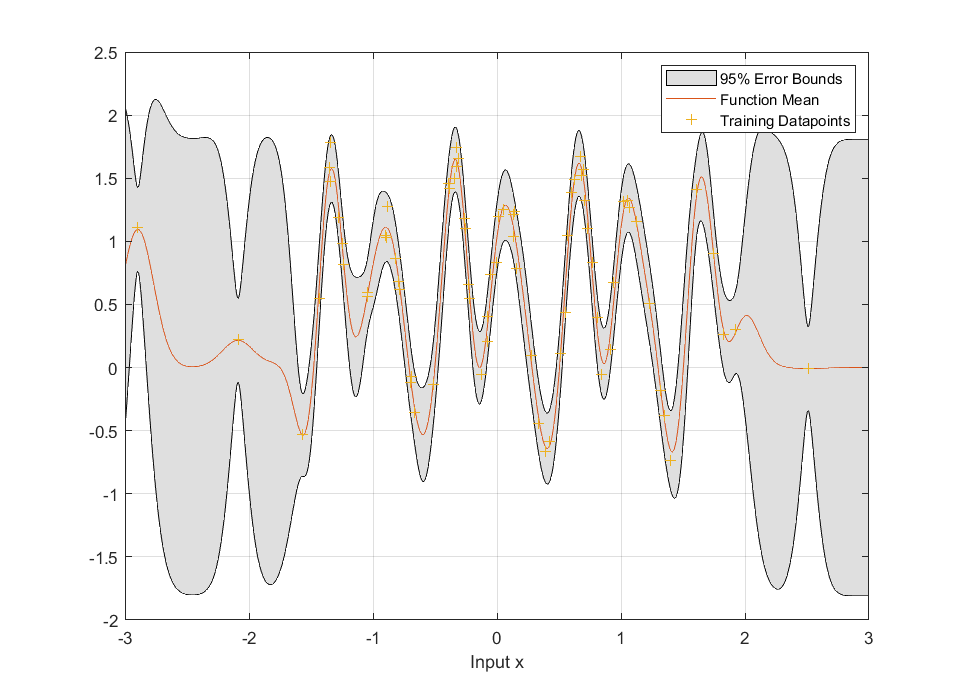
\includegraphics[width=\linewidth]{1a}
		\caption{Basic hyperparameter initialisation}
		\label{fig:1a}
	\end{subfigure}
	\begin{subfigure}{0.5\linewidth}
		\centering
		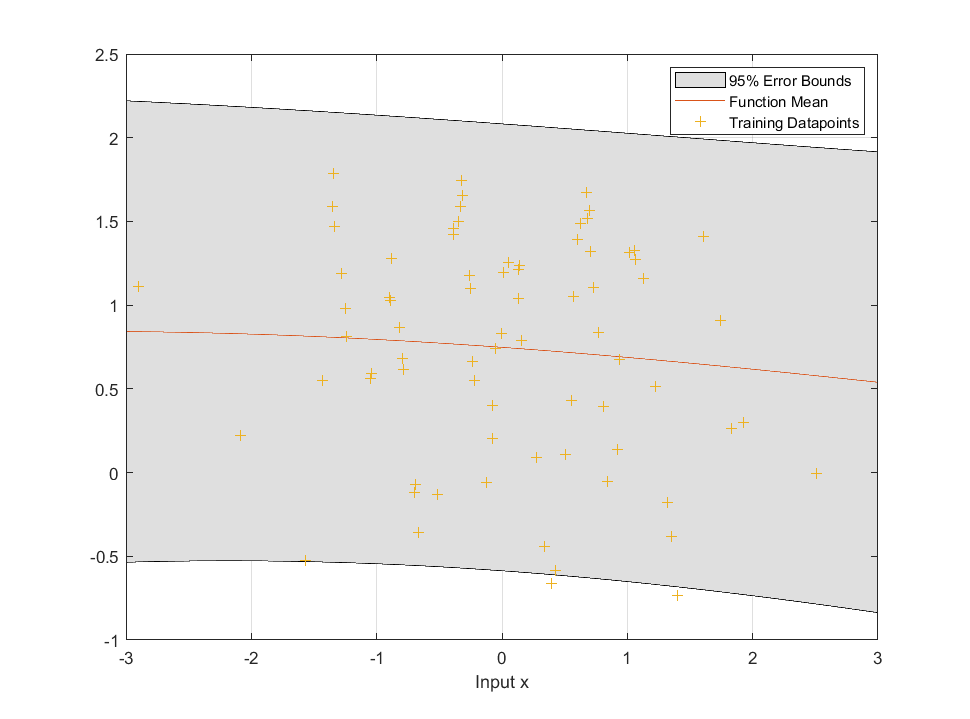
\includegraphics[width=\linewidth]{1b}
		\caption{Alternative hyperparameter initialisation}
		\label{fig:1b}
	\end{subfigure}
	\caption{Squared Exponential covariance Gaussian Process trained on data}
	\label{fig:1}
\end{figure}

We see that the error bars are always centred on the mean and that they have small standard deviations for regions in which we have many datapoints observed. This makes intuitive sense as we cannot make confident predictions in areas where the training data is sparse (such as for $|x| \geq 3$). The hyperparameters do not change enormously form the optimisation. We have that the length scale of variation $\lambda$ shrinks slightly to 0.128 - which agrees with the length scale of variation in the dataset. The scale factor $\nu$ also shrinks slightly to 0.897 as the model is able to match the data quite accurately. Indeed, the noise variance $\sigma$ shrinks significantly from 1 to 0.118 meaning the error bars are quite narrow in regions of high data density (the error bars remain large outside these regions as we are uncertain in the value of the mean function).

\subsection{Hyperparameter Initialisation}

However, the optimisation only finds a local minimum of the negative log-likelihood $\Lcal$. Therefore, a different intialisation of the hyperparameters can yield different results. This is illustrated in scenario B of table \ref{tab:hyp-opt}. It was found that an initial value of $\log \lambda = -0.45$ was a critical point. Any setting of $\log \lambda$ above this would converge to the case-B optimum; anything below converges to the original case-A optimum. Varying $\nu$ only seemed to change the position of this critical point but would not converge to an altogether different solution.

This alternative optimum (B) converges to a very large value of the length scale $\lambda=8.045$. This model expects data to vary very slowly with respect to $x$ and indeed attributes all variation within the observed range to noise. Indeed, figure \ref{fig:1b} shows that the mean varies little over the data range. Indeed, the error bars remain nearly constant and very large. This parameter setting does not seem to fit the data well just by comparing figures \ref{fig:1a} and \ref{fig:1b}. This intuition can be quantified through the marginal log-likelihood. Parameter setting B has a far larger $\Lcal$, ($\Lcal_B=78.2 >> 11.9 = \Lcal_A$) so we can conclude that B is much more unlikely.


\subsection{Periodic Covariance Function}

We can instead use a periodic covariance function to model the data (as in equation \ref{eqn:covPeriodic}. We introduce a new parameter $\rho$ which is the period of the repetition in covariance. $\lambda$ should no longer be thought of as a length scale but rather sets the strength of the correlation between neighbours and $\nu$ sets the baseline variance.

\begin{equation}
k_{PER}(x, x') = \nu^2 \exp
\left\{
- \frac{2 \sin ^2 \left( \pi (x-x') / \rho \right)}{\lambda^2}
\right\}
\label{eqn:covPeriodic}
\end{equation}

We tune the hyperparameters in much the same way as before; the results are summarised in table \ref{tab:per}. All hyperparameters stay close to their initial values. Indeed, the period $\rho$ stays very close to 1.

\begin{table}[!h]
\centering
\begin{tabular}{c | c c}
	\textbf{Parameter} & \textbf{Initial} & \textbf{Final} \\ \hline
	$\log \lambda$     & 0                & 0.0437         \\
	$\lambda$          & 1                & 1.044          \\
	$\log \rho$        & 0                & -0.0012        \\
	$\rho$             & 1                & 0.999          \\
	$\log \nu$         & 0                & 0.2122         \\
	$\nu$              & 1                & 1.24           \\ 
	$\log \sigma$      & 0                & -2.213         \\
	$\sigma$           & 1                & 0.109          \\ \hline
	$\Lcal$            & 79.5             & -35.3
\end{tabular}
\caption{Periodic covariance function hyperparameter tuning}
\label{tab:per}
\end{table}

We can plot the predictions on figure \ref{fig:1c} which shows excellent agreement between model and data. Indeed, the error bars are uniformly small. On first inspection this appears to be a more natural fit than the squared exponential covariance function. However, we must be careful to avoid overfitting.

\begin{figure}[!h]
	\centering
	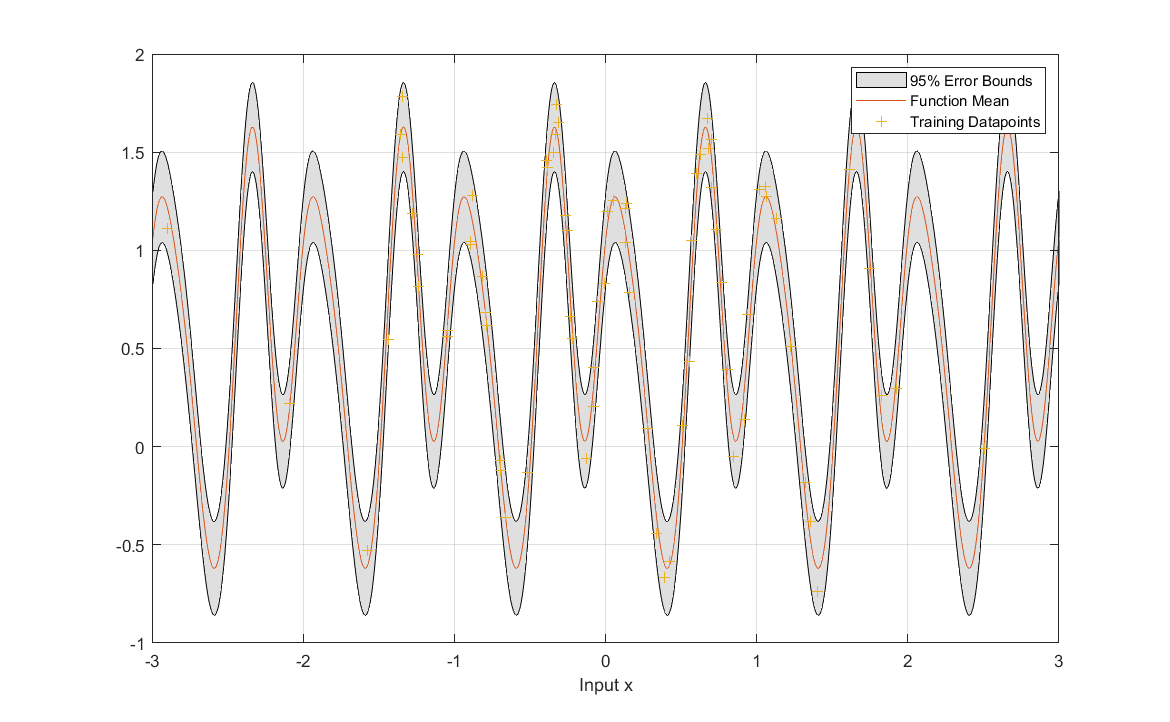
\includegraphics[width=\figwidth]{1c}
	\caption{Periodic covariance GP on same training data}
	\label{fig:1c}
\end{figure}

Indeed, the noise standard deviation $\sigma$ is slightly smaller for the periodic covariance model. Nevertheless, it does not appear that the training data was generated in a periodic manner. On figure \ref{fig:1c1}, we plot a histogram of the training inputs. This appears Gaussian with zero mean and modest variance $O(1)$. Therefore, it is highly unlikely that the data was generated in a periodic manner across the range [-3, 3]. We prefer the model in part a (SE covariance) as this remains uncertain in areas of sparse data.

\begin{figure}[!h]
	\centering
	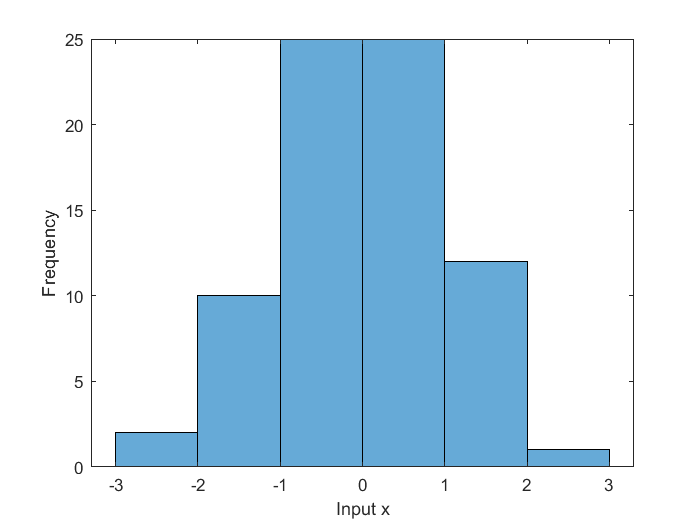
\includegraphics[width=\figwidth]{1c1}
	\caption{Histogram of training inputs}
	\label{fig:1c1}
\end{figure}

\subsection{Sampling from a Gaussian Process}

We can sample from an arbitrary GP at a finite array of points $\mathbf{x}$ by evaluating the covariance matrix $K$ for these points and exploiting the Cholesky Decomposition ($\text{chol}(K) = C$ s.t. $C C^T = K$). The code for this is in listing \ref{lst:gp-sampling}. We must add a small diagonal matrix to ensure that $K$ is positive definite and thus has a Cholesky decomposition.

\begin{lstlisting}[frame=single, caption={GP sampling}, label={lst:gp-sampling}]
x = linspace(-5, 5, n)';
z = gpml_randn(seed, n, 1);
K = feval(covfunc{:}, cov, x);
K_pos_def = K + 1e-6 * eye(n);
y = chol(K_pos_def)'*z;
\end{lstlisting}

We use this code to sample from a GP with composite covariance function defined as the product of a periodic covariance function and a standard Squared Exponential covariance function. The hyperparameters are set to $[\lambda, \rho, \nu]_{PER} = [0.607, 1, 1]$ for the periodic component and $[\lambda, \nu]_{SE} = [7.39, 1]$ for the SE component. We can run the code in \ref{lst:gp-sampling} for different values of the seed to yield the set of plots in figure \ref{fig:1d}.

\begin{figure}[!h]
	\begin{subfigure}{0.3\linewidth}
		\centering
		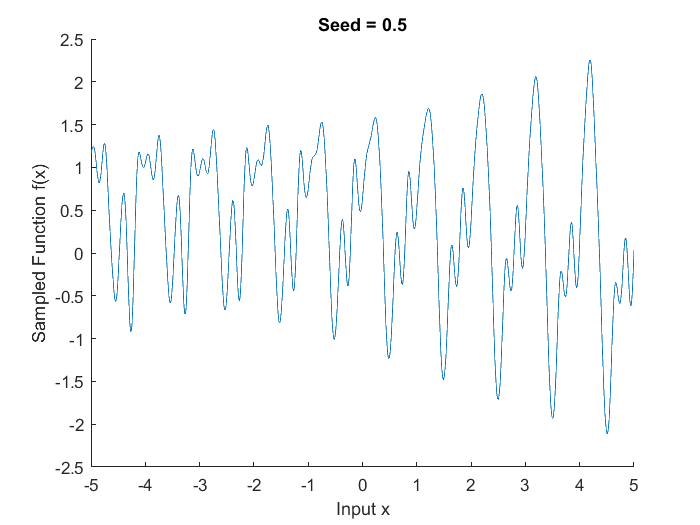
\includegraphics[width=\linewidth]{1d1}
		\caption{Seed = 0.5}
		\label{fig:1d1}
	\end{subfigure}
	\begin{subfigure}{0.3\linewidth}
		\centering
		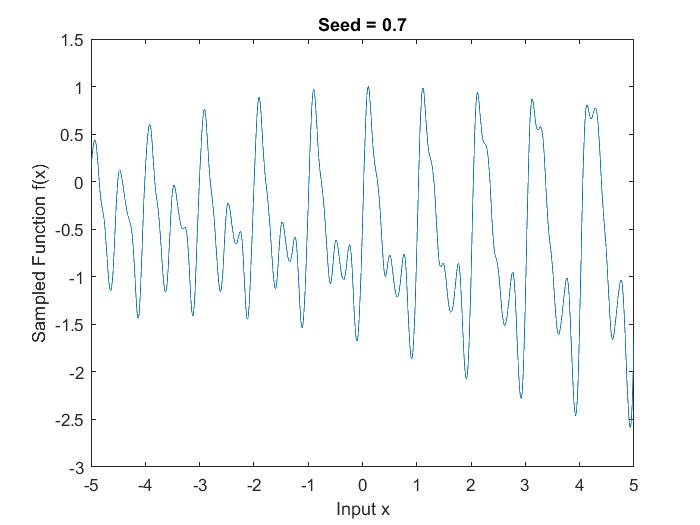
\includegraphics[width=\linewidth]{1d2}
		\caption{Seed = 0.7}
		\label{fig:1d2}
	\end{subfigure}
	\begin{subfigure}{0.3\linewidth}
		\centering
		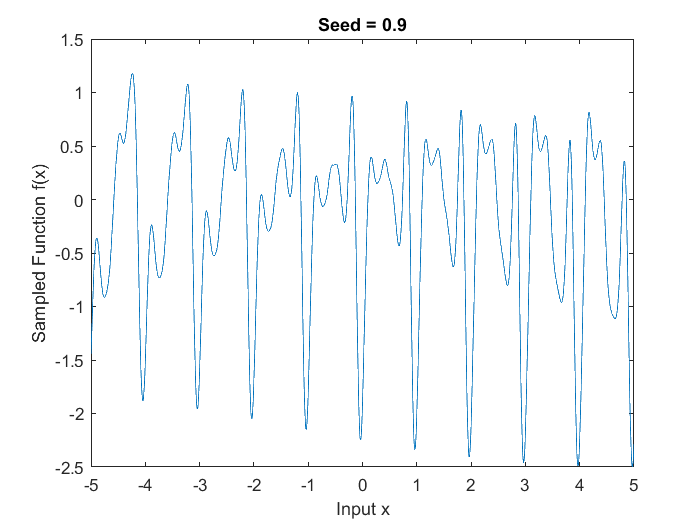
\includegraphics[width=\linewidth]{1d3}
		\caption{Seed = 0.9}
		\label{fig:1d3}
	\end{subfigure}
	\caption{Sampling function at random from a GP with composite product periodic and SE covariance}
	\label{fig:1d}
\end{figure}

This set of characteristic functions share some key properties. The functions do appear in some way periodic with period 1. This agrees with the hyperparameter setting $\rho_{PER}=1$. The SE component has a very long length scale $\lambda_{SE}=7.39$ This means that we only see distortion of the periodic structure over long length scales; adjacent periods are very similar but those that are further apart have different form.

\subsection{2-Dimensional Input - Model Comparison}

We now extend our investigation to deal with 2-dimensional input data. For this we need a new covariance function. For the simple case we choose a Squared Exponential - Automatic Relevance Determination (SE-ARD) covariance function. This is in general anisotropic and has formula given by equation \ref{eqn:covSEard}. The index $i$ iterates through every dimension in our input (total $D$ dimensions). In this example, the data is 2-dimensional ($D=2$).

\begin{equation}
k_{ARD}(\mathbf{x}, \mathbf{x}') = \nu^2 \exp\left\{- \frac{1}{2} \sum_{i=1}^{D}\frac{(x_i-x_i')^2}{\lambda_i^2}\right\}
\label{eqn:covSEard}
\end{equation}

We wish to compare this simple model with a more complex model. The covariance functions for the simple and additive model are given in equations \ref{eqn:cov-a} and \ref{eqn:cov-b} respectively.The vector $\theta = [\nu, \lambda_1, \lambda_2]$ denotes the hyperparameters of the SE-ARD covariance function.

\begin{equation}
k^a(\mathbf{x}, \mathbf{x}') = k_{ARD}(\mathbf{x}, \mathbf{x}' ; \theta^a)
\label{eqn:cov-a}
\end{equation}
\begin{equation}
k^b(\mathbf{x}, \mathbf{x}') = k_{ARD}(\mathbf{x}, \mathbf{x}' ; \theta^{b1})
+ k_{ARD}(\mathbf{x}, \mathbf{x}' ; \theta^{b2})
\label{eqn:cov-b}
\end{equation}

\begin{table}[!h]
	\centering
	\subfloat[Simple model a]{
		\begin{tabular}{c | c c}
			\textbf{$\theta^a$} & \textbf{Initial} & \textbf{Final} \\ \hline
			$\log \lambda_1$         & 0                & 0.413          \\
			$\lambda_1$              & 1                & 1.511          \\
			$\log \lambda_2$         & 0                & 0.252          \\
			$\lambda_2$              & 1                & 1.287          \\
			$\log \nu$         & 0                & 0.102          \\
			$\nu$              & 1                & 1.107          
		\end{tabular}
	}
	\subfloat[Component b1]{
		\begin{tabular}{c | c c}
			$\theta^{b1}$ & \textbf{Initial} & \textbf{Final} \\ \hline
			$\log \lambda_1$         & 0                & 0.3644         \\
			$\lambda_1$              & 1                & 1.440          \\
			$\log \lambda_2$         & 0                & 6.3200         \\
			$\lambda_2$              & 1                & 555.6          \\
			$\log \nu$         & 0                & 0.0801         \\
			$\nu$              & 1                & 1.083        
		\end{tabular}
	}
	\subfloat[Component b2]{
		\begin{tabular}{c | c c}
			$\theta^{b1}$ & \textbf{Initial} & \textbf{Final} \\ \hline
			$\log l_1$         & 0                & 6.000          \\
			$l_1$              & 1                & 403.4          \\
			$\log l_2$         & 0                & -0.0072        \\
			$l_2$              & 1                & 0.993          \\
			$\log \nu$         & 0                & -0.3351        \\
			$\nu$              & 1                & 0.715        
		\end{tabular}
	}
	\caption{Parameter optimisation for 2-D data}
	\label{tab:simple-opt}
\end{table}

\begin{figure}[!h]
	\begin{subfigure}{0.5\linewidth}
		\centering
		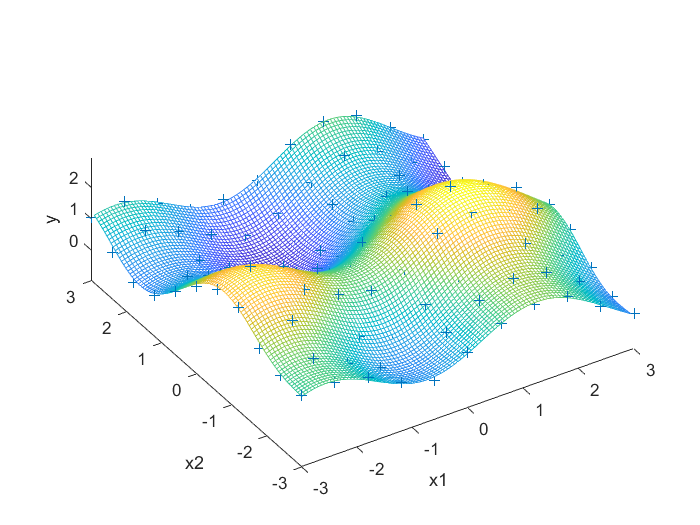
\includegraphics[width=\linewidth]{1e1}
		\caption{Basic covariance function: single covSEard model}
		\label{fig:1e1}
	\end{subfigure}
	\begin{subfigure}{0.5\linewidth}
		\centering
		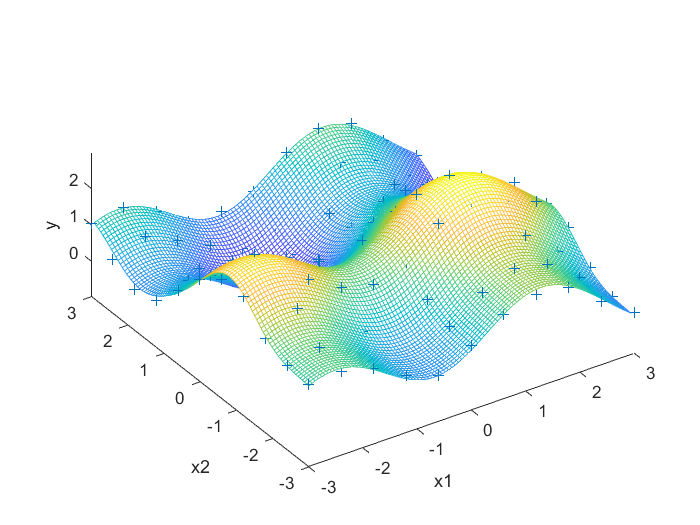
\includegraphics[width=\linewidth]{1e2}
		\caption{Additive covariance function: two covSEard model}
		\label{fig:1e2}
	\end{subfigure}
	\caption{Comparison of two covariance function fits on training data}
	\label{fig:1e}
\end{figure}

\begin{figure}[!h]
	\begin{subfigure}{0.5\linewidth}
		\centering
		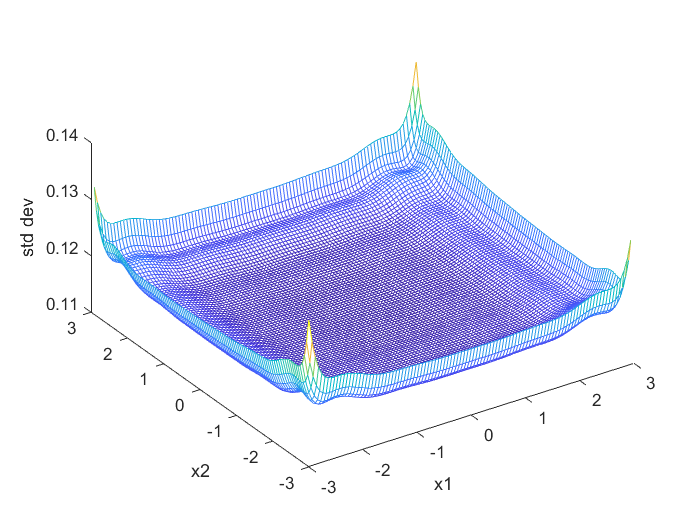
\includegraphics[width=\linewidth]{1e1b}
		\caption{Basic covariance function: single covSEard model}
		\label{fig:1e1}
	\end{subfigure}
	\begin{subfigure}{0.5\linewidth}
		\centering
		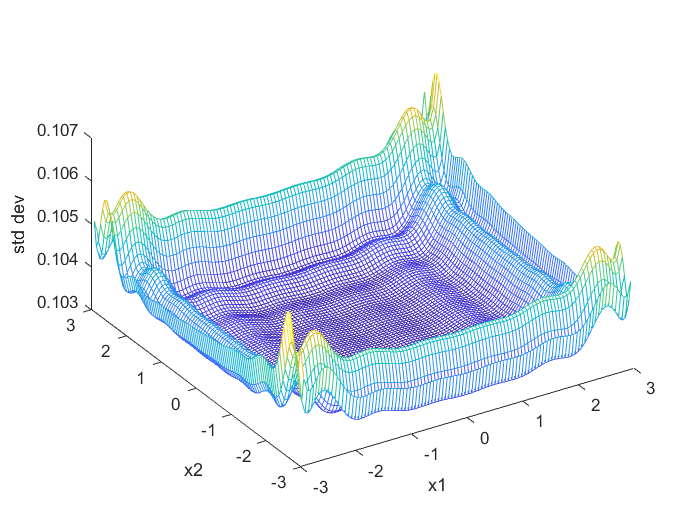
\includegraphics[width=\linewidth]{1e2b}
		\caption{Additive covariance function: two covSEard model}
		\label{fig:1e2}
	\end{subfigure}
	\caption{Comparison of standard deviation for }
	\label{fig:1e}
\end{figure}


\end{document}
